%\subsection{Sensitivity to heavy Higgs bosons from the 2HDM in "Higgs-to-Higgs" decays}

\begin{center}
 {K. Mimasu$^{1}$, J. M. No$^{2}$ \\
}
%\noindent
 {\small $^{1}$Universite catholique de Louvain, Chemin du Cyclotron, 2, B-1348 Louvain-la-Neuve, Belgium \\
 $^{2}$Departamento de Fisica Teorica and Instituto de Fisica Teorica, IFT-UAM/CSIC, Cantoblanco, 28049, Madrid, Spain}
\end{center}

\vspace{2mm}

Searches for heavy scalars are highly complementary to coupling measurements of the 125 GeV Higgs $h$ as probes of extended Higgs sectors. 
Di-boson search channels $H \to WW$, $ZZ$ probe the parameter space for which the 125 GeV Higgs is not SM-like, 
in combination with Higgs coupling measurements. Both probes suffer suffer a significant loss in  
sensitivity to new physics in the limit of a SM-like 125 GeV Higgs, 
since the couplings $HVV$ ($V = W^{\pm},\,Z$) vanish in such case.
For two-Higgs-doublet-model (2HDM) scenarios, this corresponds to the so-called alignment limit~\cite{Gunion:2002zf},
where searches for heavy scalars through non-standard ``Higgs-to-Higgs"
decay channels~\cite{Coleppa:2014hxa,Dorsch:2014qja,Li:2015lra,Kling:2016opi,Dorsch:2016tab} 
as well as through fermionic decay channels~\cite{Craig:2015jba,Gori:2016zto} become a key avenue to find these new states, 
and are crucial to fully cover the parameter space of 2HDMs.

We focus here on HL-LHC and HE-LHC probes of neutral scalars via ``Higgs-to-Higgs" decays, and briefly discuss also their interplay 
with direct searches of such states in fermionic decay channels. Specifically, we consider a general 2HDM scalar potential with a softly broken 
$\mathbb{Z}_2$ symmetry (and no CP violation), given by 
%
\begin{eqnarray}	
\label{2HDM_potential}
V(H_1,H_2) &= &\mu^2_1 \left|H_1\right|^2 + \mu^2_2\left|H_2\right|^2 - \mu^2\left[H_1^{\dagger}H_2+\mathrm{h.c.}\right] 
+\frac{\lambda_1}{2}\left|H_1\right|^4 +\frac{\lambda_2}{2}\left|H_2\right|^4 \nonumber \\
&+& \lambda_3 \left|H_1\right|^2\left|H_2\right|^2
+\lambda_4 \left|H_1^{\dagger}H_2\right|^2+ \frac{\lambda_5}{2}\left[\left(H_1^{\dagger}H_2\right)^2+\mathrm{h.c.}\right]\, . 
\end{eqnarray}
%
Apart from the 125 GeV Higgs $h$, the 2HDM scalar sector includes two neutral states 
$H$ and $A$, respectively CP-even and CP-odd, as well as a charged scalar $H^{\pm}$.
Regarding the couplings of the two doublets $H_{1,2}$ to fermions, we consider  
a Type-I and a Type-II 2HDM scenarios (see e.g.~\cite{} for a review),
with the parameters $t_{\beta} \equiv \mathrm{tan}\,\beta$ and $c_{\beta -\alpha} \equiv \mathrm{cos}\,(\beta-\alpha)$ controlling 
the coupling strength of the various 2HDM scalars to gauge bosons and fermions.
% 

Focusing on the 2HDM neutral scalars, the decay $A \to Z H$ ($H \to Z A$) yields a powerful probe of the 
region $m_A > m_H + m_Z$ ($m_H > m_A + m_Z$)~\cite{Coleppa:2014hxa,Dorsch:2014qja}. 
We first obtain the present 13 TeV LHC limits on the 2HDM parameter space from the 
search $A \to Z H$ ($Z\to \ell\ell$, $H \to b\bar{b}$) by ATLAS with $36.1$ fb$^{-1}$~\cite{Aaboud:2018eoy} (see also~\cite{Khachatryan:2016are,CMS:2016qxc} for 
corresponding searches by CMS), considering in particular the alignment limit $c_{\beta -\alpha} = 0$.
Our signal cross sections and branching fractions are obtained 
respectively with {\sl SusHi}~\cite{Harlander:2012pb} and {\sl 2HDMC}~\cite{Eriksson:2009ws}, and we use the 
publicly available observed 95 $\%$ C.L. signal cross section limits in the ($m_A$, $m_H$) plane from~\cite{Aaboud:2018eoy}.   
In order to derive a sensititivy projection of this search to HL-LHC and HE-LHC with 
$3000$ fb$^{-1}$ of integrated luminosity, we first perform a $\sqrt{\mathcal{L}}$ rescaling of the present ATLAS expected 
sensititivy, assuming that the background uncertainties are statistically dominated.
We then perform a further rescaling of the sensitivity from $\sqrt{s} = 13$ TeV to 
$\sqrt{s} = 14$ TeV (HL-LHC) and $\sqrt{s} = 27$ TeV (HE-LHC) under the assumption that the
ratio of acceptance$\times \sigma$ for the SM background for 27 TeV, 14 TeV and 13 TeV are the
same as the ratio of Higgs production cross section\footnote{That is, we assume signal and background increase by the same amount in going from 
13 TeV to 14 TeV, or 13 TeV to 27 TeV. This is a conservative assumption particularly for high masses $m_A$.}. 
The present bounds and projected sensitivities are shown in Figure~\ref{AZH_HL-LHC} in the 
($m_A$, $\mathrm{tan}\beta$) plane for Type I (left) and Type II (right) 2HDM, 
considering respectively $m_A = m_H + 100$ GeV (top) and $m_A = m_H + 200$ GeV (bottom).
We note that, since the limits from~\cite{Aaboud:2018eoy} do not extend beyond 
$m_A = 800$ GeV or go below $m_H = 130$ GeV, our corresponding projections based on those limits cannot 
extend beyond those parameter regions either. 
 

\begin{figure}[h]
\begin{center}
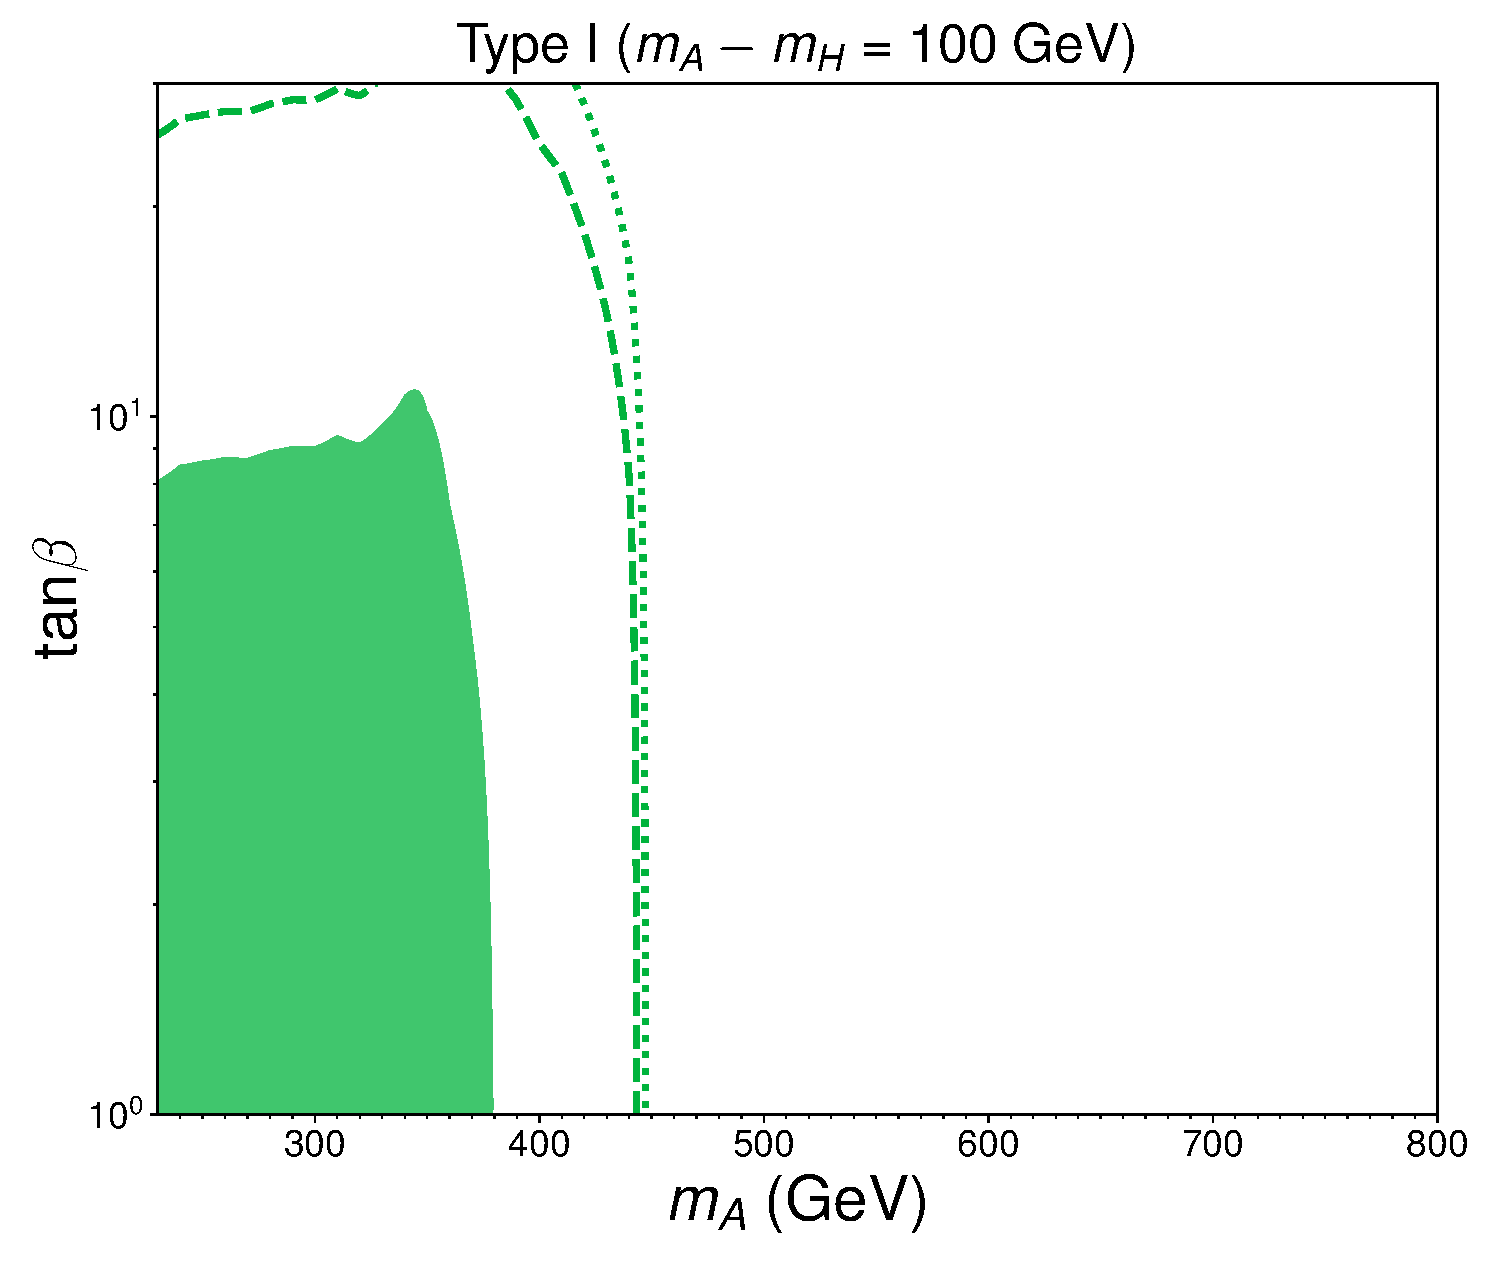
\includegraphics[width=0.4\textwidth]{\main/section9/plots/2HDM_AZH_Type1_100.pdf}
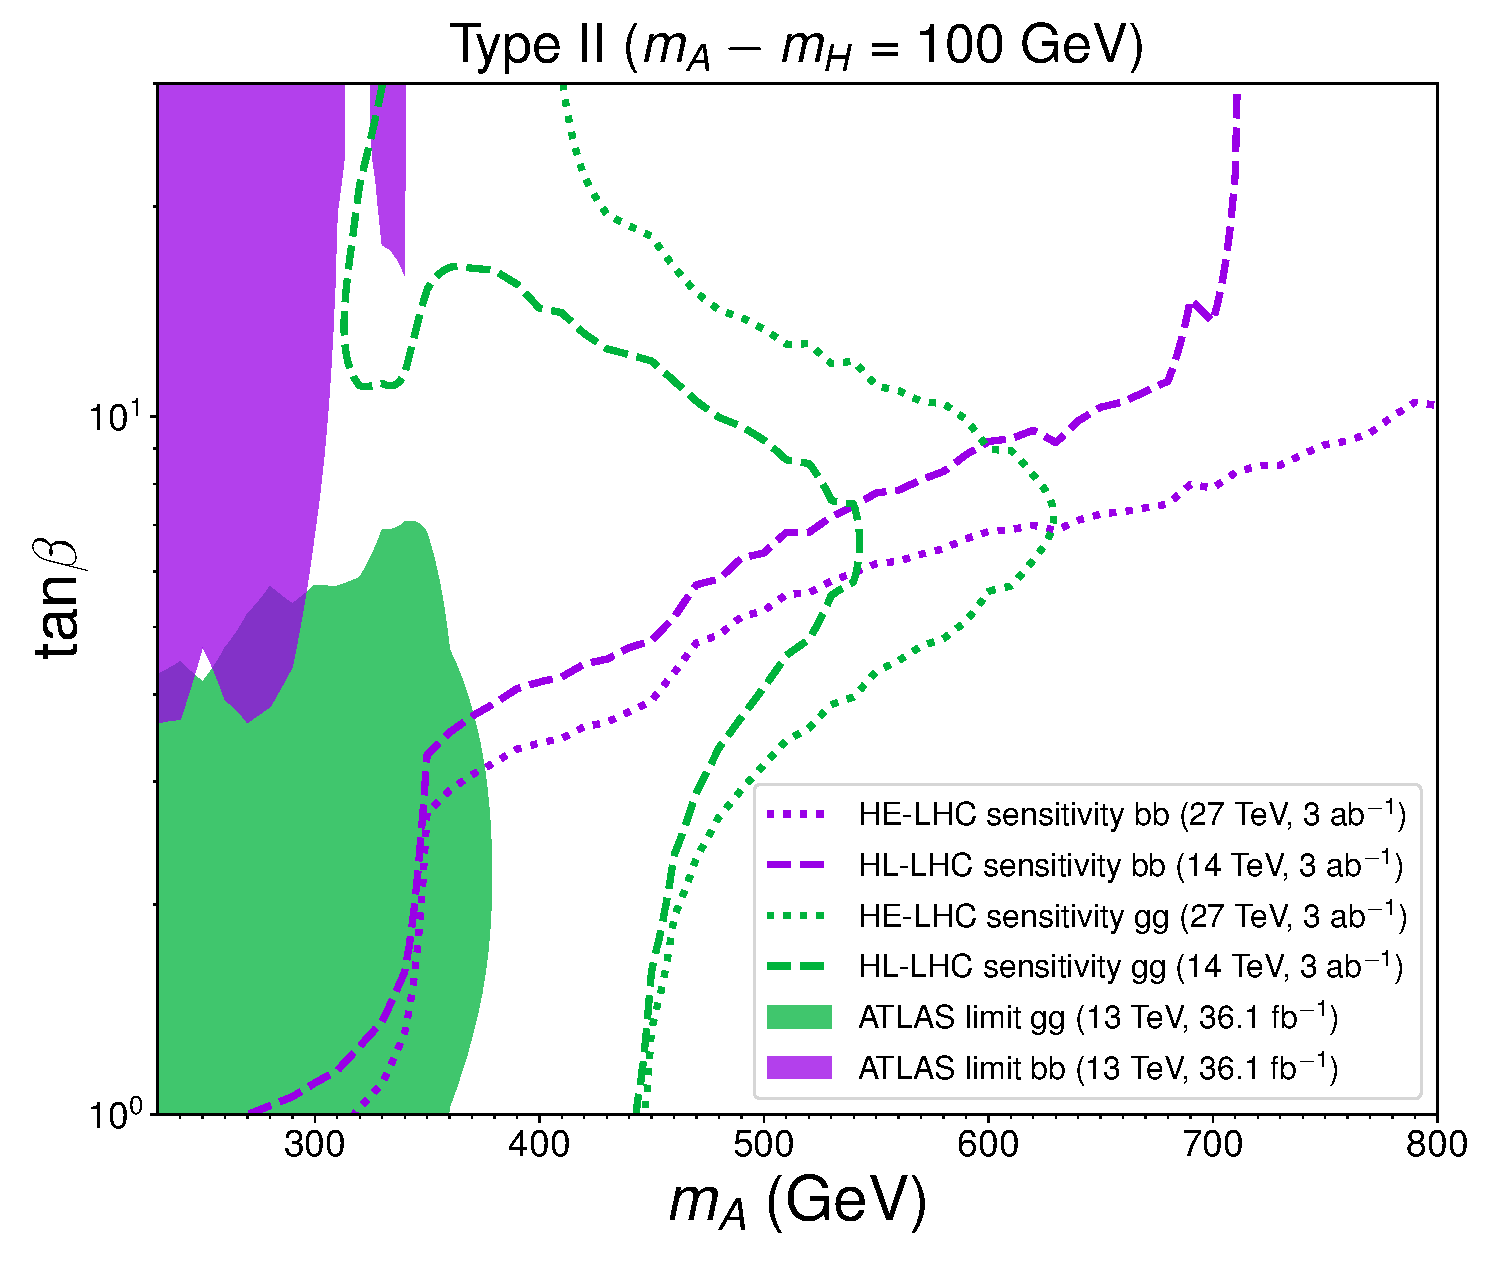
\includegraphics[width=0.4\textwidth]{\main/section9/plots/2HDM_AZH_Type2_100.pdf}
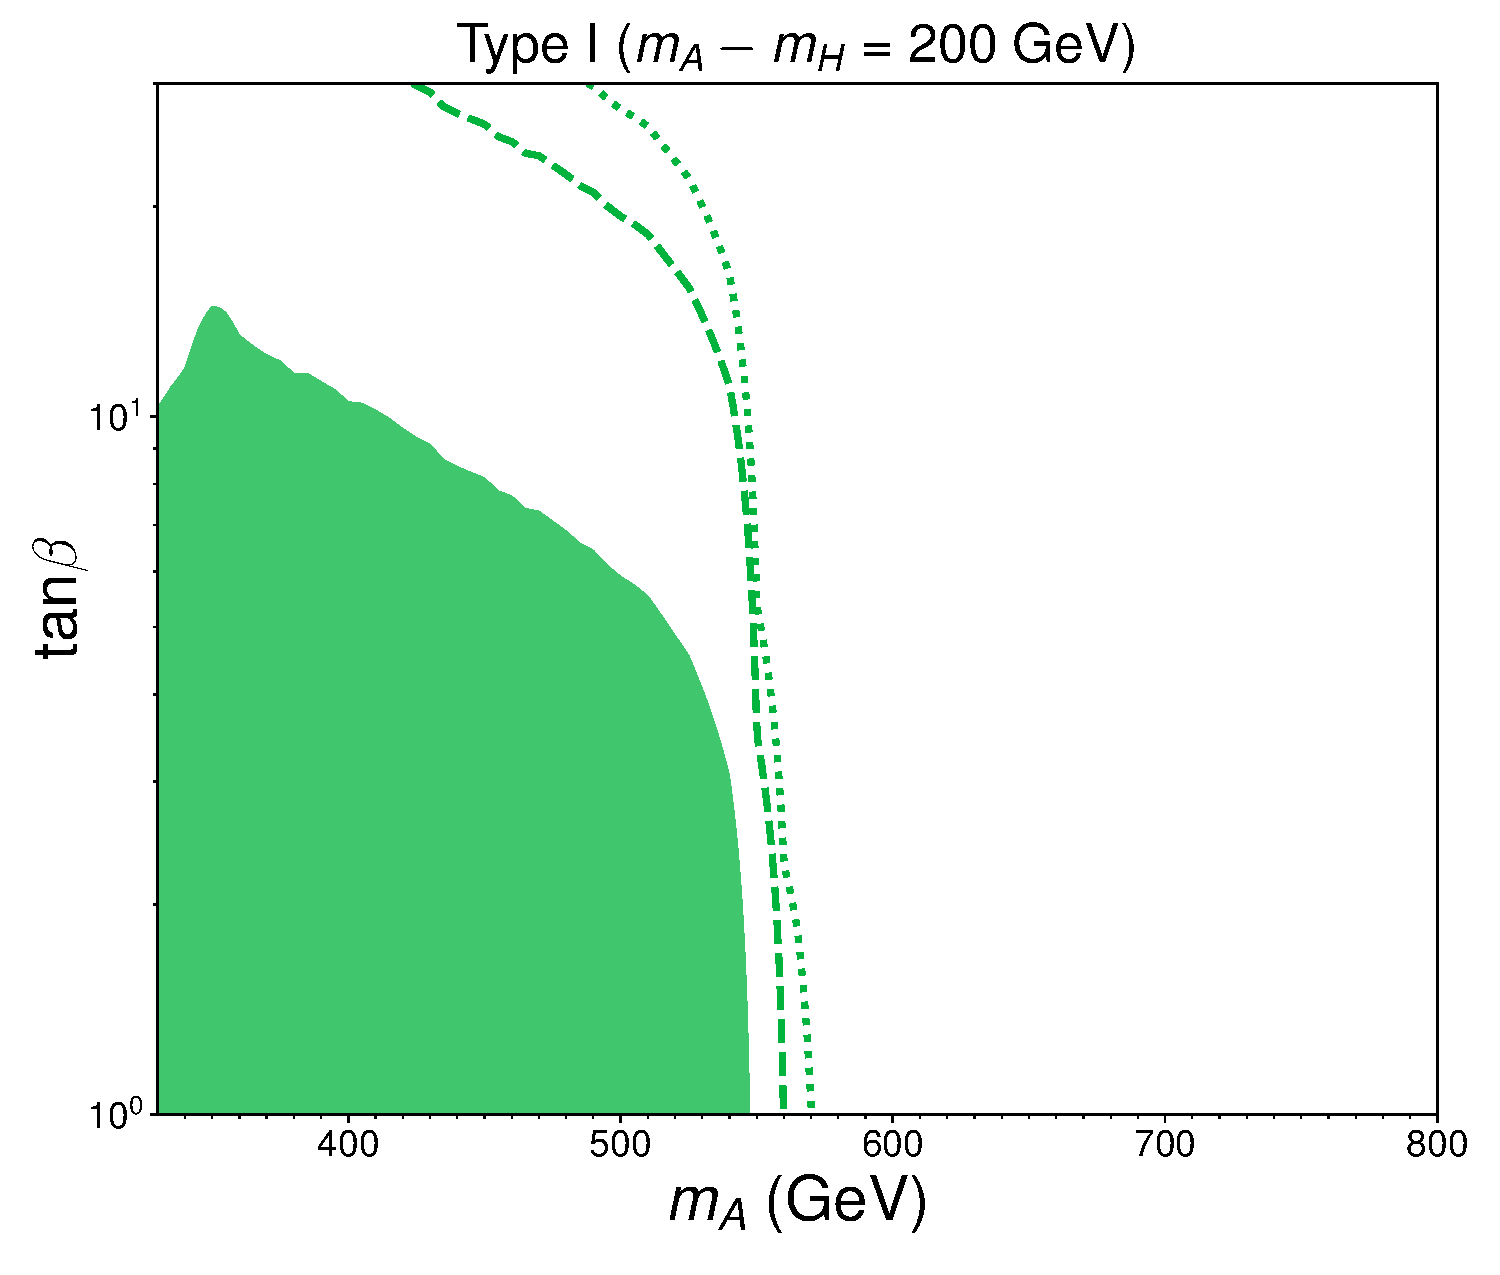
\includegraphics[width=0.4\textwidth]{\main/section9/plots/2HDM_AZH_Type1_200.pdf}
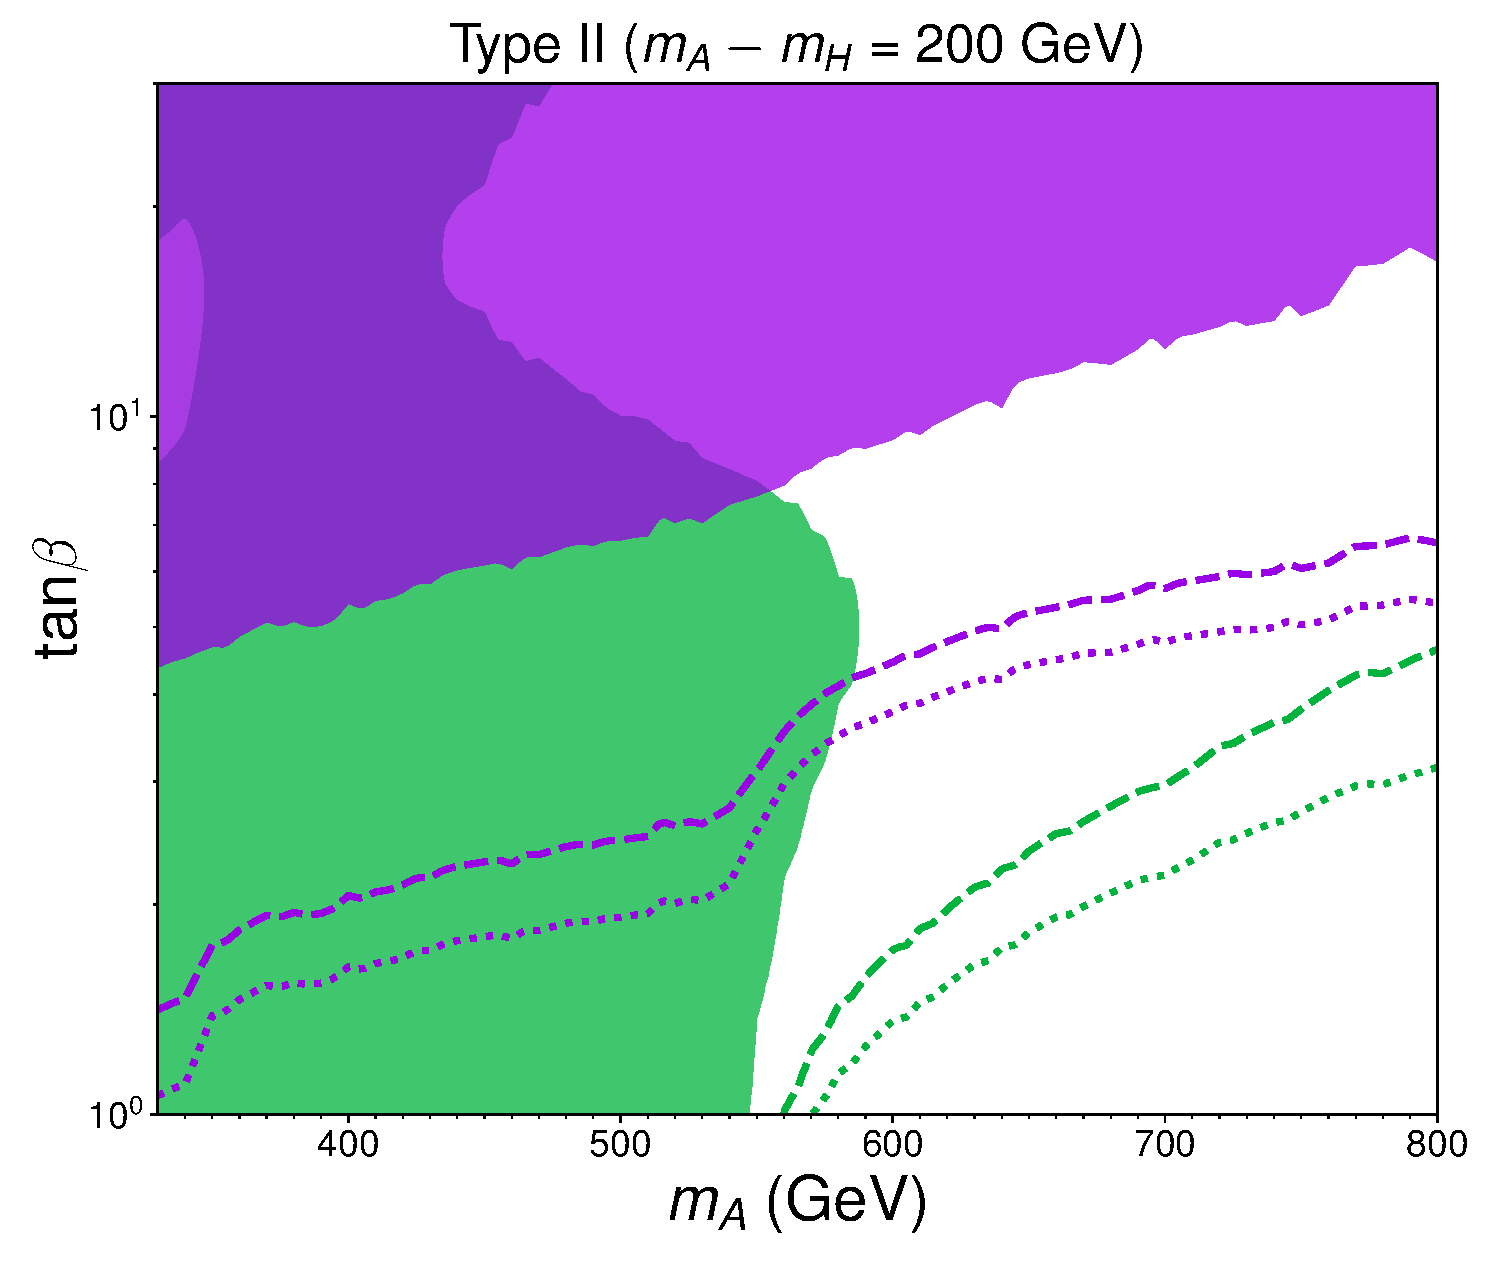
\includegraphics[width=0.4\textwidth]{\main/section9/plots/2HDM_AZH_Type2_200.pdf}
\caption{\small Present (solid), projected for 14 TeV HL-LHC with $3000$ fb$^{-1}$ (dashed) and projected for HE-LHC with $3000$ fb$^{-1}$ (dotted)
$95\%$ C.L. exclusion sensitivity for $p p \to A \to Z H \to \ell\ell b \bar{b}$  
in the ($m_{A}$, tan$\beta$) plane for 2HDM Type I (left) and 2HDM Type II (right), for $m_A = m_H +100$ GeV (top) and 
$m_A = m_H +200$ GeV (bottom), from 
gluon fusion (orange) and $bb$-associated production (blue).}
\label{AZH_HL-LHC}
\end{center}
\end{figure}

In order to study the interplay of the above searches with heavy scalar searches in fermionic decay modes like $H/A \to \tau\tau$, 
we translate the model-independent HL-LHC and HE-LHC sensitivity projections for $\phi \to \tau\tau$ from section (9.6.3) 
to the $m_{\phi}$, $\mathrm{tan}\beta$ plane (with $\phi = H/A$) of the 2HDM (here assume one scalar at a time? should be a fair assumption if 
$|m_A - m_H| \gg \delta m_{\tau\tau}$, with $\delta m_{\tau\tau}$ the invariant mass resolution of the analysis)
using {\sl SusHi}~\cite{Harlander:2012pb} and {\sl 2HDMC}~\cite{Eriksson:2009ws}, assuming 
$\mathrm{cos}(\beta - \alpha) = 0$.
